% TO-DO:

\input{../YKY-preamble.tex}

\usepackage{color}
\usepackage{mathtools}
\usepackage{hyperref}

\usepackage[backend=biber,style=authoryear]{biblatex}
\bibliography{../AGI-book}
% \renewcommand*{\bibfont}{\footnotesize}

\usepackage{graphicx} % Allows including images
\usepackage{tikz-cd}
\usepackage{tikz}
\usepackage[export]{adjustbox}% http://ctan.org/pkg/adjustbox
\usepackage{verbatim} % for comments
% \usepackage{tikz-cd}  % commutative diagrams
% \newcommand{\tikzmark}[1]{\tikz[overlay,remember picture] \node (#1) {};}
% \usepackage{booktabs} % Allows the use of \toprule, \midrule and \bottomrule in tables
% \usepackage{amssymb}  % \leftrightharpoons
% \usepackage{wasysym} % frownie face
% \usepackage{newtxtext,newtxmath}	% Times New Roman font
% \usepackage{sansmath}

\numberwithin{equation}{section}

\newcommand{\underdash}[1]{%
	\tikz[baseline=(toUnderline.base)]{
		\node[inner sep=1pt,outer sep=10pt] (toUnderline) {#1};
		\draw[dashed] ([yshift=-0pt]toUnderline.south west) -- ([yshift=-0pt]toUnderline.south east);
	}%
}%

\DeclareSymbolFont{symbolsC}{U}{txsyc}{m}{n}
\DeclareMathSymbol{\strictif}{\mathrel}{symbolsC}{74}

\newcommand{\highlight}[1]{\colorbox{pink}{$\displaystyle #1$}}

\newcommand{\emp}[1]{{\color{violet}\textbf{#1}}}
\newcommand*\confoundFace{$\vcenter{\hbox{\includegraphics[scale=0.2]{../confounded-face.jpg}}}$}

\newcommand*{\Cdot}{\raisebox{-0.5ex}{\scalebox{2}{$\cdot$}}}
\newcommand{\witness}{\scalebox{0.6}{$\blacksquare$}}
% \newcommand{\Heytingarrow}{\mathrel{-}\mathrel{\triangleright}}
\providecommand\Heytingarrow{\relbar\joinrel\mathrel{\vcenter{\hbox{\scalebox{0.75}{$\rhd$}}}}}

\begin{document}

\title{\cc{\bfseries\color{blue}{\Huge Logic in Hilbert space}}
{{\Huge Logic in Hilbert space}}}
\author{YKY \\{\small general.intelligence@gmail.com}} % Your name
%\institute[] % Your institution as it will appear on the bottom of every slide, may be shorthand to save space
%{
%Independent researcher, Hong Kong \\ % Your institution for the title page
%\medskip
%\textit{generic.intelligence@gmail.com} % Your email address
%}
\date{\today} % Date, can be changed to a custom date

\maketitle

\section*{Summary}
\begin{itemize}
	\item It seems possible to construct a model of the \textbf{untyped} $\lambda$-calculus in Hilbert space, with function application $f(g)$ implemented as $\llbracket g \rrbracket \circ \llbracket f \rrbracket$.
	
	\item Doing so allows \textbf{self-application} of logic predicates (Curry's paradox can be avoided by the fuzzy truth value ``don't know'')
	
	\item The use of \textbf{continuous maps} may be advantageous in machine-learning because \textbf{generalization} seems to work best with ``continuous'' domains (as opposed to maps acting on symbolic logic representations which may be discontinuous).

	\item Elements in the infinite-dimensional $\mathcal{H}$ can be realized on a computer as \textbf{neural networks} (which are functions $\mathbb{R}^n \rightarrow \mathbb{R}^n$ \textbf{finitely} generated from sets of weights).
\end{itemize}

% \tableofcontents
% \vspace*{0.5cm}
% 多谢 支持 \smiley

\setcounter{section}{-1}
\section{Inspiration}

In the 1960's Dana Scott constructed a model for untyped $\lambda$-calculus, using a domain $D_{\infty}$ with the property $D_{\infty}^{D_{\infty}} \cong D_{\infty}$.  This started off the field known as \textbf{domain theory}.

Scott initially believed that such models cannot exist, but later discovered that they can be constructed.  In retrospect, this is not surprising because the Church-Rosser theorem demonstrated that the untyped $\lambda$-calculus is consistent.

Scott's idea is to begin with an initial domain $D_0$ and define $D_{n+1}$ to be the function space $D_n \rightarrow D_n$.

Thus it is guaranteed, for any domain $d \in D_{\infty}$, one can always find a function space $d \rightarrow d$.  Therefore the space $D_{\infty}$ is isomorphic to $ D_{\infty} \rightarrow D_{\infty}$.

That this claim does not contradict Cantor's theorem (a set $X$ cannot be isomorphic to $X^X$) is because the functions are restricted to \textbf{continuous} maps, sending open sets to open sets, also known as Scott-continuous (these are not \textit{all} the functions in $X \rightarrow X$).

The detailed definition of $D_{\infty}$ involves building a cumulative hierarchy of infinite sequences, with pairs of operators $\psi_n, \Psi_n$ going up and down levels.  For a gentle exposition one may read \parencite{Stenlund1972}, Ch.1 \S6.

\section{Requirements}

In order to define a logical calculus in $\mathcal{H}$, what we need are:
\begin{itemize}
	\item a family of functions dense in $\mathcal{H}$
	\item self-application:  maps can act on other maps; how to define $f(g)$?
	\item define the $\mathbf{S}, \mathbf{K}, \mathbf{I}$ combinators in combinatory logic
 	\item how does an element $e \in \mathcal{H}$ translate to and from a (syntactic) logic formula?
\end{itemize}

\section{Elements in $\mathcal{H}$}

The structure of $D_{\infty}$ is reminescent of Cantor's ordinal number $\varepsilon_0$:
\begin{equation}
{\displaystyle \varepsilon _{0}=\omega ^{\omega ^{\omega ^{\cdot ^{\cdot ^{\cdot }}}}}=\sup\{\omega ,\omega ^{\omega },\omega ^{\omega ^{\omega }},\omega ^{\omega ^{\omega ^{\omega }}},\dots \}}
\end{equation}
but this number is still ``smaller'' than the \textbf{continuum}, ie. the real line $\mathbb{R}$.  This led me to think that models of $\lambda$-calculus may be found in the Hilbert space of continuous functions.

But such a Hilbert space would be $\infty$-dimensional.  Next I consider the \textbf{neural network} as a function $f$:
\begin{eqnarray}
\mathbb{R}^n & \stackrel{f}{\longrightarrow} & \mathbb{R}^n \\
x & \mapsto & y \nonumber
\end{eqnarray}
and notice that $f$ and $x, y$ are ``unequal'' because $f$ can \textbf{act on} $x, y$ but not the other way round.  This is partly because $f$ is $\infty$-dimensional whereas $x, y$ are finite-dimensional.  So, what if we increase $n$ to $\infty$, then perhaps $x, y$ would become the same kind of objects as $f$ ?  In an informal sense $\mathcal{H}$ is $\mathbb{R}^{\infty}$.

The Universal Approximation theorem of \parencite{Cybenko1989} (with later extensions by others) states that the family of neural networks is \textbf{dense} in the space of continuous functions, with respect to the supremum norm.  This means that we have a nice way of generating elements in $\mathcal{H}$ that can be finitely represented in a computer.

\section{Function application}

Now we lack the notion of a function \textbf{applying} to another function, such as $f(g)$.  Since we only need the functions as elements of $\mathcal{H}$, the domains $\mathbb{R}^n$ is somewhat ``immaterial''.  We might as well assume $\mathbb{R}^n$ to be common among all functions (the dimension $n$ can be fixed for implementation considerations), and thus function \textbf{composition} such as $f \circ g$ always exists.  So we define:
\begin{equation}
\llbracket f(g) \rrbracket = \llbracket g \rrbracket \circ \llbracket f \rrbracket
\end{equation}
where $\llbracket \Cdot \rrbracket$ denotes ``model of''.  (The reversed order $g \circ f$ is to prepare for dealing with tuples; see below.)

\section{Combinatory logic in $\mathcal{H}$}

We need to implement the combinators defined by:
\begin{eqnarray}
\mathbf{I} x &=& x \nonumber \\
\mathbf{K} x y &=& x \\
\mathbf{S} x y z &=& xz (yz) \nonumber 
\end{eqnarray}
which obviously requires that some functions take on $> 1$ arguments.  So we need the notion of \textbf{tuples} and of functions applying to tuples.

\subsubsection*{Tuples}

We can implement tuples like $(g, h)$ simply by stacking them vertically:
\begin{equation}
(g, h) = \begin{bmatrix}
g \\
h
\end{bmatrix}
\end{equation}
which is a $\mathbb{R}^{2n} \rightarrow \mathbb{R}^{2n}$ function.  This can be extended to dimension $kn$.  Function application can be implemented as:
\begin{equation}
\llbracket f(g, h) \rrbracket =
\begin{bmatrix}
\llbracket g \rrbracket \\
\llbracket h \rrbracket
\end{bmatrix} \circ \llbracket f \rrbracket
\end{equation}
where $f$ is of type $\mathbb{R}^{2n} \rightarrow \mathbb{R}^n$.  We can visualize the right hand side like this:
\begin{equation}
\begin{tikzcd}[column sep=small, row sep=-0.5em]
g \arrow[-, dr] & & \\
& f \arrow[-, r] & {} \\
h \arrow[-, ur] & &
\end{tikzcd} 
\end{equation}

\subsubsection*{Interpreting logic formulas}

It is helpful to bear in mind that a functional form
\begin{equation}
f(g, h) = e
\end{equation}
in Hilbert space corresponds to a logic formula
\begin{equation}
g \wedge h \stackrel{f}{\Longrightarrow} e
\end{equation}
where $f$ plays the role of an \textbf{implication}, or logical \textbf{consequence}, $g \wedge h \vdash e$.  In fact $f$ encodes the \textit{entire} formula $g \wedge h \Rightarrow e$, but even more than that, $f$ can be applied to other arguments.  (Readers may recognize that the function $f$ realizes an implication statement in logic via the \textbf{Curry-Howard isomorphism}.)

With tuples, we can easily implement the combinators $\mathbf{S}, \mathbf{K}, \mathbf{I}$.  The treatment for $\lambda$-calculus would be analogous, and I would add that to a later version of this paper when I have time.

\subsubsection*{Arities}

There is a remaining problem with arities.  Because we allow tuples, compositions with tuples leave us with functions with arity $> 1$.  For example, the following two applications of $f$ yield the same result $c$, and we would like to make these definitions of $f$ consistent:
\begin{eqnarray}
\begin{tikzcd}[column sep=small, row sep=-0.5em]
a \arrow[-, dr] & & \\
& f \arrow[-, r] & c\\
b \arrow[-, ur] & &
\end{tikzcd} 
& \qquad f(a,b) = c \\
\begin{tikzcd}[column sep=small]
d \arrow[-, r] & f \arrow[-, r] & c
\end{tikzcd} 
& \qquad f(d) = c
\nonumber 
\end{eqnarray}
but the \textbf{arity} of $f$ appears different in the equations.  My solution is to adjoin a \textbf{null} input to the single input, that is:
\begin{equation}
\begin{tikzcd}[column sep=small, row sep=-0.5em]
d \arrow[-, dr] & & \\
& f \arrow[r] & c\\
\varzero \arrow[-, ur] & &
\end{tikzcd}
\qquad f(d, \varzero) = c
\end{equation}
In implementation, this can be done ``on demand'', as the number of conjunctions in the premise of a logic rule is usually a small number.

\section{Usage as AI logic}

Usually there would be a ``big'' neural network, representing a special function $f$, that plays the role of a \textbf{knowledge base}, consisting of (the conjunction of) a huge number of logic rules of the form $\Gamma \vdash \Delta$.  This $f$ would send various logic formulas to their conclusions, for a single inference step.  In this sense $f$ embodies all the \textit{knowledge} in the AI system.

What is special with this Hilbert-space model is that we can now construct arbitrary logic formulas as elements in $\mathcal{H}$, which can be acted upon by $f$.

For example, ``if we touch fire we may get burnt'' is a logic formula of the form $A \Rightarrow B$.  In a primitive AI (or animal), this formula is \textit{implicitly} stored in the transition function $f$, which performs the logic inference $A \vdash B$.  The animal or AI has no conscious reckoning of $A \Rightarrow B$.  Now with Hilbert space we can create an element $A \Rightarrow B$, ie. an object that can \textbf{participate} in logic inference.  We can take arbitrarily complex logic formulas and have them represented as Hilbert space elements.

A simple logic formula such as $A \Rightarrow B$ is a \textbf{section} of the big map $f$ restricted to the domain $A$.  In this case, the restricted function is \textbf{degenerate} and is in effect just a pair $(A, B)$.  Also, a single atomic proposition, eg. $A$, can be implemented as $\top \Rightarrow A$, a trick commonly used in Prolog.

\section{Conclusion}

I am not highly confident of this invention, as its technical details are a bit complicated (We could build a simpler AI using a big neural network to act on \textit{symbolic} logic formulas; indeed the BERT model is a case in point).  If human-level intelligence turns out to be very hard to learn by an AGI, at least we can turn to this, more powerful approach.

Questions, comments welcome \smiley

Dana Scott (1932-) and S\"{o}ren Stenlund (1943-2019):
\begin{equation}
\vcenter{\hbox{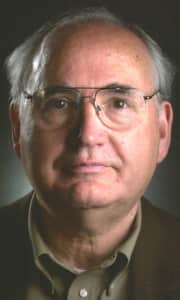
\includegraphics[scale=1]{Dana-Scott.jpg}}} \qquad
\vcenter{\hbox{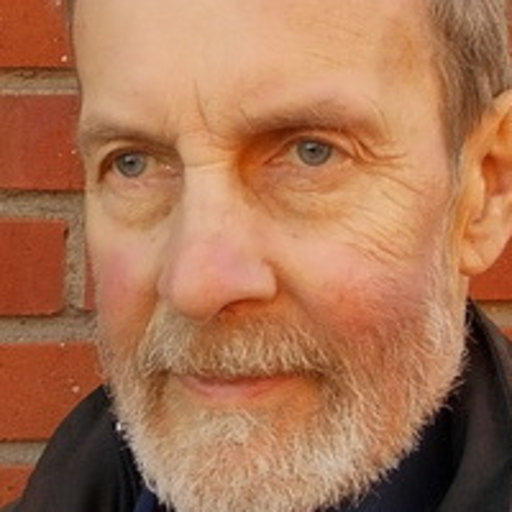
\includegraphics[scale=0.35]{Stenlund.jpg}}} \nonumber
\end{equation}

\printbibliography

\end{document} 
